\section{Case Study} \label{sec:casestudy}
We present a case study used as a motivating example in this paper. Figure \ref{fig:warehouse} is a snapshot of a warehouse environment where packages need to be moved from shelves to a loading area to be sent for delivery. UAVs also need to periodically visit a charging station. 
\begin{figure}
\centering
\subfloat[Warehouse simulation environment in ROS.]{
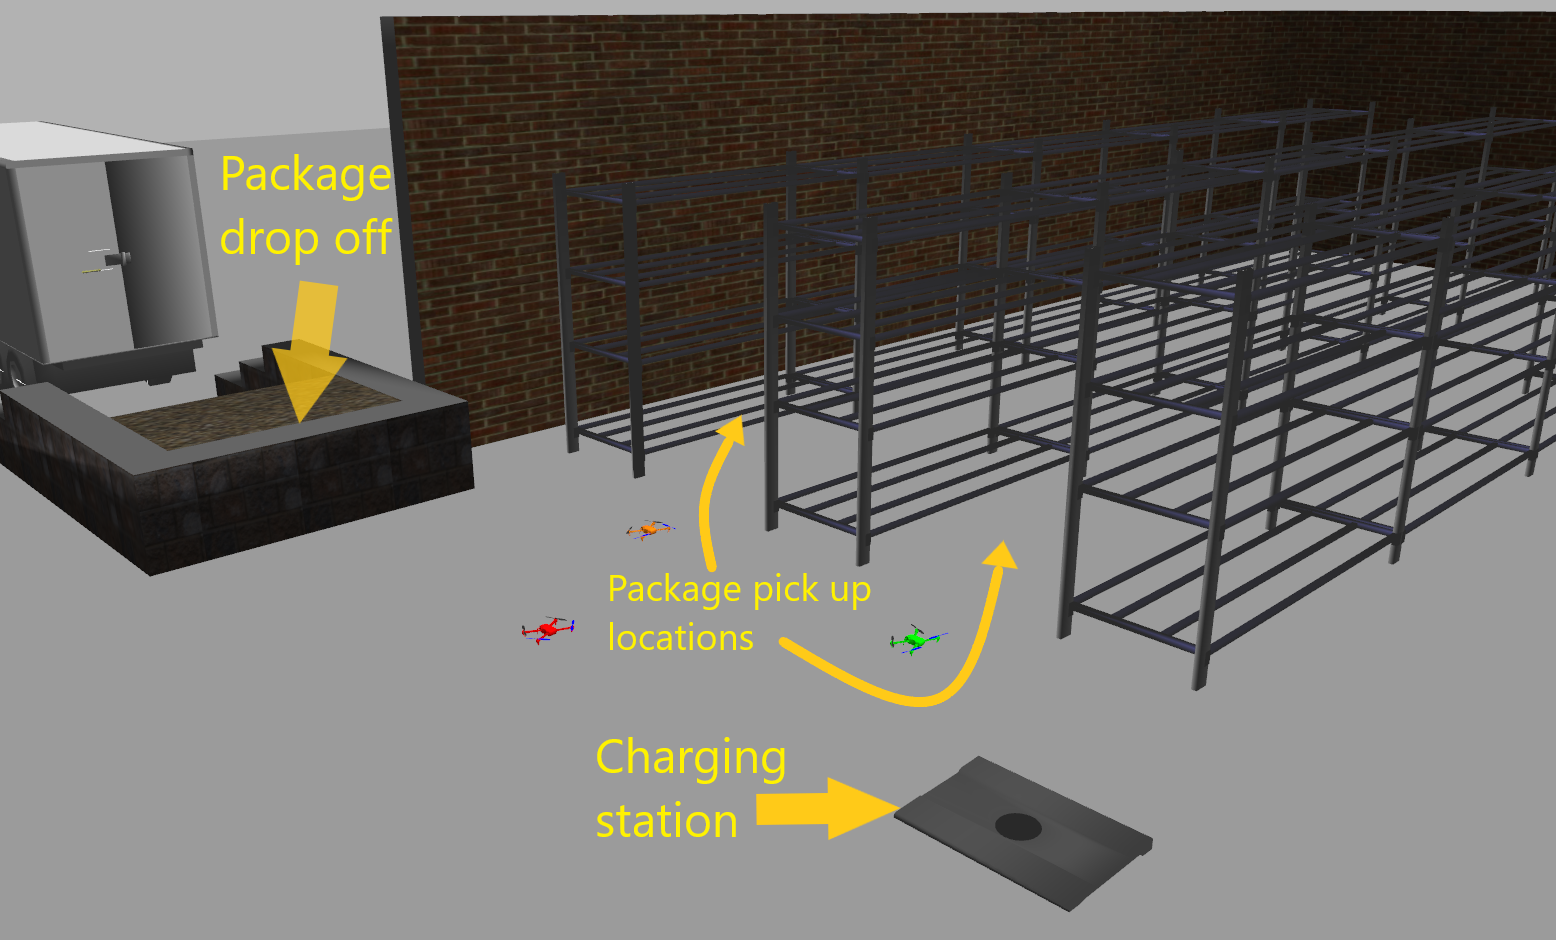
\includegraphics[width=0.75\textwidth]{MultiShield/figs/arenapicwithpad}
%\caption{Warehouse simulation environment in ROS.}
\label{fig:warehouse}
}
\hfill
\subfloat[Flowchart of the composed system.]{
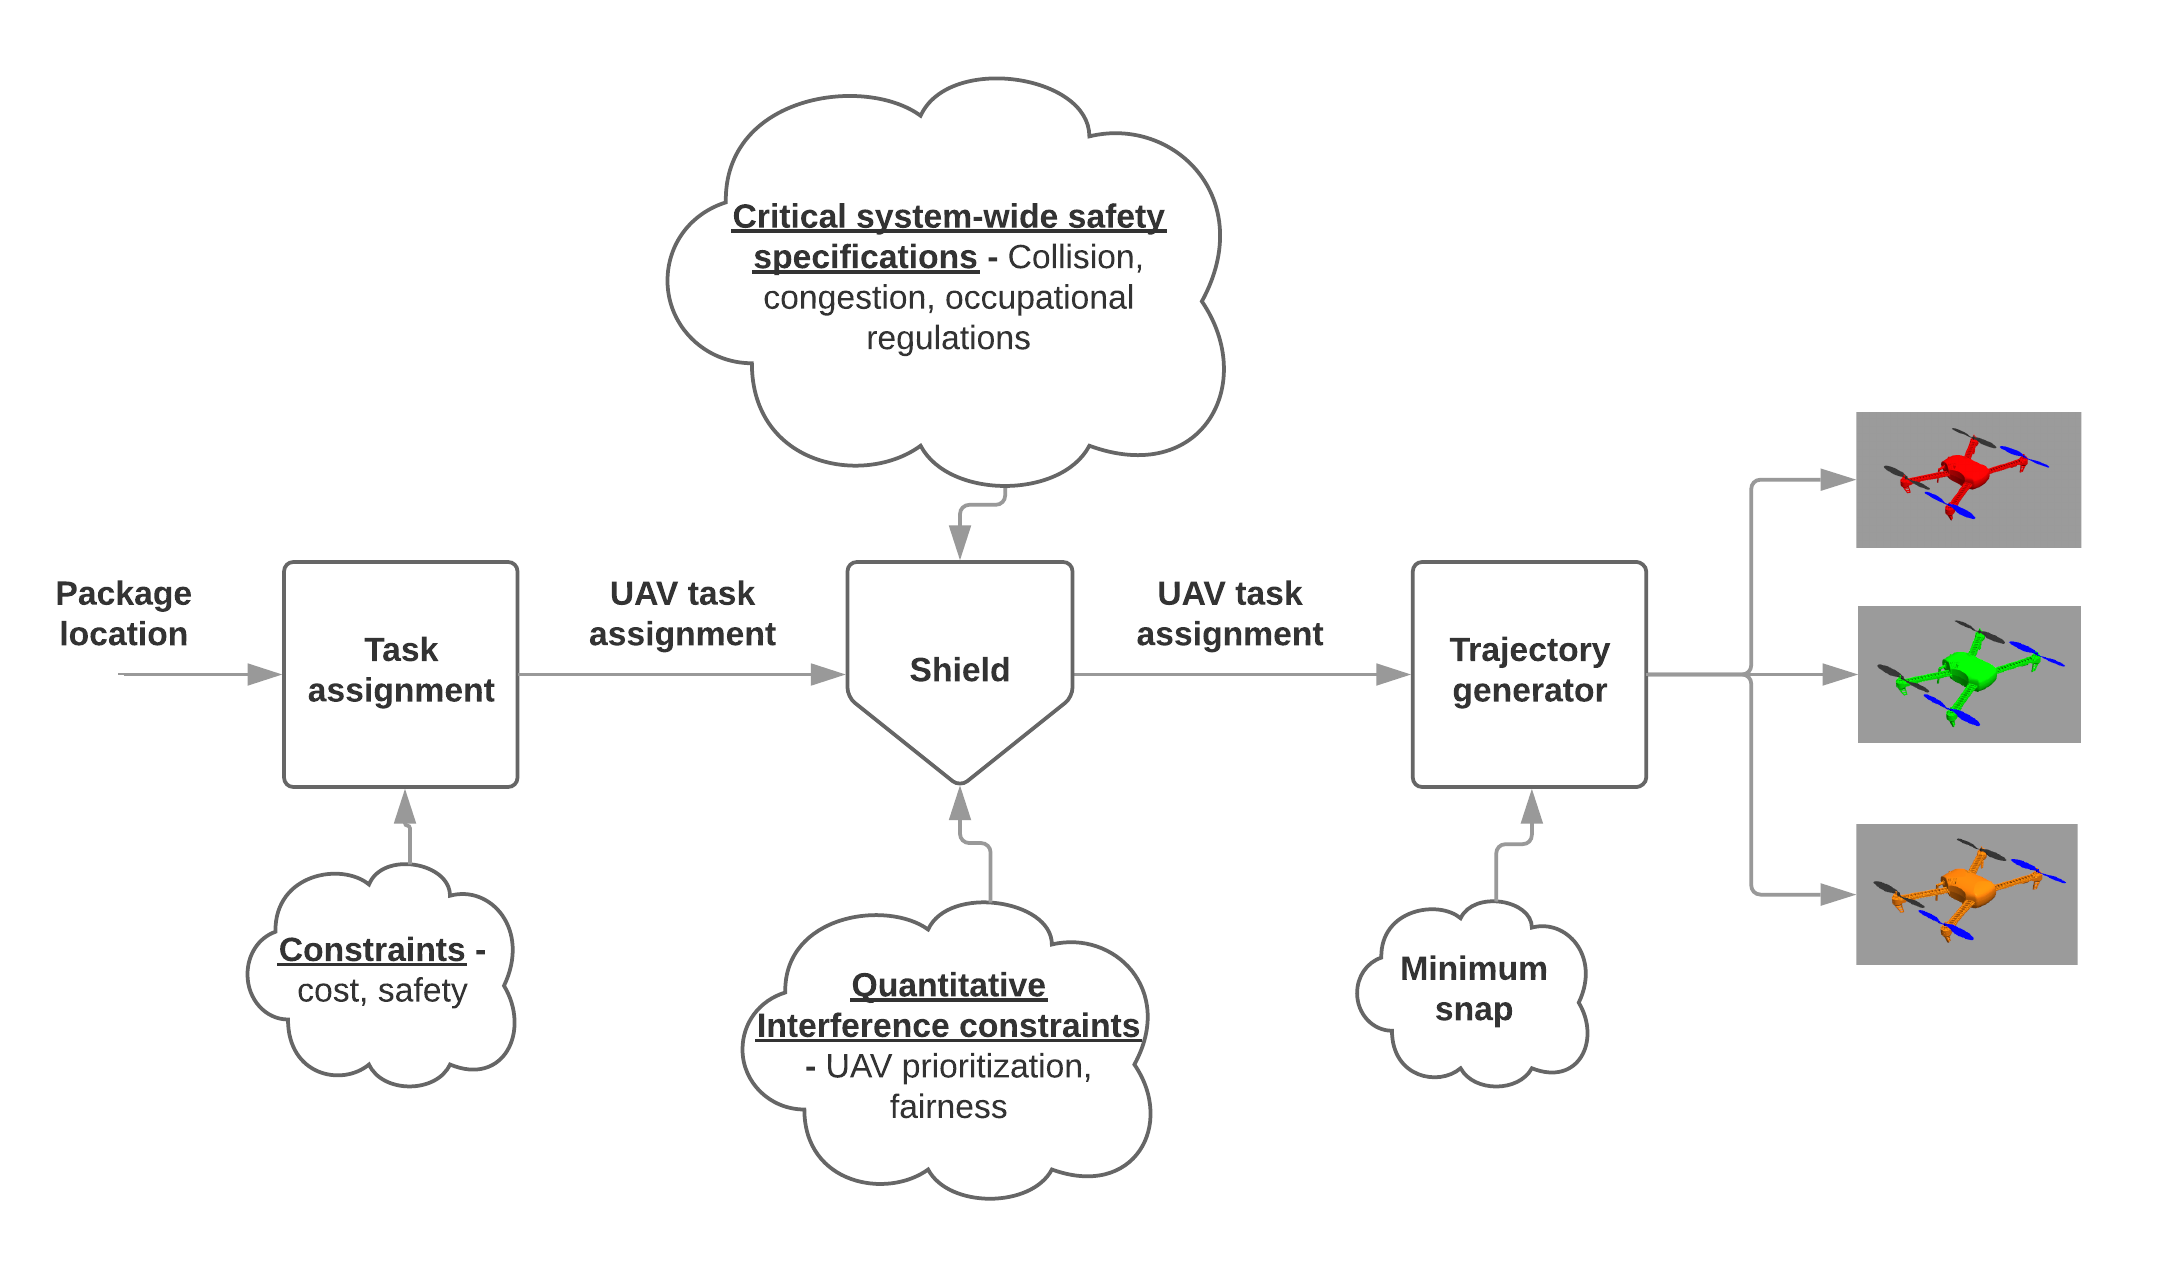
\includegraphics[width=0.7\textwidth]{MultiShield/figs/casestudy}
\label{fig:flowchart}}
\caption{Simulation environment and process workflow for three UAVs tasked with picking up packages off shelves and delivering them to the loading area.}
\label{fig:casestudy}
\end{figure}

The commands sent to move package(s) from the shelves to the loading dock are used to generate task assignments for the UAVs, and constitute the input to the system. The task assignment for the UAVs is sent either by a human operator who can command a particular UAV to perform a certain task, or by an automated system such as those in \cite{olivo2016method,kalyan2015automated}. To prevent congestion and collisions, global requirements for the multi-UAV system include not allowing more than one UAV in a given row at the same time, not allowing the UAVs to fly too close to each other, and not allowing UAVs to charge or drop of packages at the same time. 

The methods proposed in this paper can be used to synthesize a shield that enforces such  global safety properties and is agnostic to the nature of the system being protected. The shield takes the task assignment as an input and overwrites it with a new task assignment when necessary.  This is then sent to a trajectory generator which generates a minimum snap trajectory for each UAV to accomplish its task. In the following sections, we present the formalization of the multi-agent shielding problem, motivated in this example.
This process is summarized in Figure \ref{fig:flowchart}. 
 
 The safety specifications for this case study, and the results of the shield synthesis procedure are described and discussed in more detail in Section~\ref{sec:results_casestudy}.

